\chapter{Solutions to the Strong \CP\ Problem}

% At first sight, the strong \CP\ problem may not appear to be a problem at all.
% After all, QCD is a theory whose Lagrangian possibly---but not necessarily---admits a term $\propto \angbr{\tsbm F \wedge \tsbm F}$ which gives rise to \CP-violating interactions in the strong force, predicting an electric dipole moment of the neutron.
% Empirical data is consistent with the neutron's electric dipole moment (and hence the \CP-violating term) being zero.
% From a phenomenological perspective, it is satisfactory to simply leave the $\bar θ$-term out of the theory's Lagrangian and end the story there.
% Indeed, a tautological way to `resolve' the strong \CP\ problem is to simply require that \CP\ be a symmetry of the strong force.
% However, this only begs the question of why \CP\ symmetry appears to be preserved in some sectors of the standard model while it is broken in others.

% Furthermore, there is a strong sense that the inclusion of the \CP-violating term is ``natural''.
% That is, we lack reason to exclude it on a theoretical basis: it is Lorentz and gauge invariant, etc.; it is a theoretical prediction of the non-trivial vacuum structure of QCD (instantons); and arises via the chiral anomaly.
% From an empirical perspective, if no \CP-violating interactions were observed in Nature, then $\bar θ$ could be justifiably set to zero on the basis of symmetry.
% However, the weak interaction is explicitly parity-violating.\footnote{
% 	In fact, the standard model is asymmetric under all combinations of charge conjugation, $C$; parity $P$; and time-reversal $T$ modulo the prevailing combined $CPT$ symmetry.
% }
% Hence, the fact that the $\bar θ$-term violates \CP\ is not theoretically satisfactory reason for its exclusion.


% % Similarly, the advent of instantons in QCD demonstrated that the $θ$-term does not necessarily vanish \cite{lectures-on-instantons,instantons-whats-happening}.\note{?????}



% The strong \CP\ problem differers from other fine-tuning problems in the standard model in the sense that it is of almost no consequence to everyday physics.
% Variation of the $θ$-parameter hardly affects nuclear physics at all because its effects are suppressed by the quark masses \cite{Dine_2018}.
% On the other hand, variations of the cosmological constant, for example, predict universes drastically different to our own, and similarly for the value of the weak scale, or the quark and lepton masses.
% Such fine-tuning problems at least have anthropic solutions---but the strong \CP\ problem does not.\footnote{
% 	Given a theory linking the presence of dark matter to the smallness of $θ$, an anthropic solution may exist if it turns out that dark matter is necessary for, e.g., galaxy formation (investigated in \cite{Dine_2018}).
% }
% % from http://scipp.ucsc.edu/~dine/solutions_of_strong_cp.pdf
% The strong \CP\ problem is therefore a compelling theoretical indication that the standard model remains incomplete.

\note{Introduce and outline solutions}


\section{The Massless Quark Solution}

The simplest resolution to the strong \CP\ problem is to stipulate that at least one quark is in fact massless.
If this were true, then $\det\mat m$ would vanish, and the parameter $\bar θ = θ + \arg\det\mat m$ would be rendered unphysical.
The \emph{massless quark solution} is the claim that $\bar θ \approx 0$ because the up quark is massless, $m_u = 0$.

% In particular, $\barθ$ becomes singular when one of the quark masses is zero.
% Therefore, the $\barθ$-parameter, and hence the $θ$-term, are entirely unphysical in the case of a massless quark.

At first sight, this economical resolution to the strong \CP\ problem appears to be in contradiction with the experimentally determined masses of the quarks, all of which are non-zero (including the up quark, with mass $\sim \SI{2.2}{\mega\eV}$).
However, it was realised in the mid-1980s that the mass of the up quark has \emph{two} contributions in the standard model Lagrangian: not only the Yukawa mass $m_u$ (the `bare mass') as introduced above, but also a non-perturbative contribution $m_\text{eff}$ from topological effects (i.e., instantons) \cite{ruling-out-massless-uquark_2020}.
Only the bare quark masses contribute to the value of $\bar θ$ via the quark mass matrix $\mat m$.
Importantly, it was plausible that this secondary source of the up quark's mass could be of order $m_\text{eff} \approx \SI{2.2}{\mega\eV}$, allowing $m_u$ to vanish while still preserving the up quark's overall mass.

The massless up quark hypothesis remained controversial until \emph{lattice gauge theory} had advanced sufficiently to made numerical simulations of non-perturbative effects in QCD possible.
Consensus was reached by 2019 that the instanton contribution $m_\text{eff}$ is not sufficiently large, and hence that the massless up quark hypothesis is false \cite{ruling-out-massless-uquark_2015,aoki2016review,ruling-out-massless-uquark_2020}.
Instead, another mechanism is required to explain the smallness of the $\barθ$-parameter.





% \section{Peccei--Quinn Theory}

% Perhaps the most famous proposed resolution to the strong \CP\ problem is the Peccei--Quinn theory of the \emph{axion}, first proposed in 1977 \cite{PecceiQuinn_1977}.
% The axion is well-known in cosmology because of the its allure as a dark matter candidate.

% Peccei--Quinn theory explains the small value of $θ$ by its promotion to a dynamical field whose potential is minimised when $\barθ = 0$.
% In other words, a new $\U(1)$ symmetry is introduced (whose action is to rotate $θ$) and is adjoined to the gauge group of QCD.
% The QCD Lagrangian is modified by the addition of a potential with minimum at $θ = 0$, which is said to \emph{spontaneously break} the Peccei--Quinn $\U(1)$ symmetry.
% The gauge field associated to this $\U(1)$ symmetry is named the \emph{axion field}, and the gauge bosons obtained upon quantisation are named \emph{axions}.

% \note{
% 	\begin{enumerate}
% 		\item Predictions of PC theory
% 		\item Theoretical limitations
% 		\item Experimental evidence
% 	\end{enumerate}
% }



\section{The Peccei--Quinn Mechanism}


Perhaps the most famous resolution to the strong \CP\ problem is the Peccei--Quinn theory of the \emph{axion}, first proposed in 1977 \cite{PecceiQuinn_1977}.
% In essence, the axion solution involves making the $\bar θ$-parameter to a field in such a way that which is dynamically relaxed to zero.
In essence, the axion solution involves extending the standard model in order to promote the original $\bar θ$-parameter to a field $\bar θ(x) = \bar θ_\text{SM} + a(x)$ in such a way that it is dynamically relaxed to zero.
In doing so, a new massive boson described by the scalar axion field $a(x)$ is necessarily introduced.
There are different inequivalent ways to extend the standard model to realise the axion solution, but all Peccei--Quinn axion models share the same necessary features:
\begin{itemize}
	\item The extended Lagrangian $\LL_\text{PQ}$ possesses an additional global chiral symmetry $\UPQ$.
	The exact action of this \emph{Peccei--Quinn symmetry} depends on the particular axion model, and is not of central importance.
	The defining feature of $\UPQ$ is that it is chiral, so that a $\UPQ$ transformation by $α$ radians anomalously induces a $θ$-term $α\angbr{\tsbm F\wedge\tsbm F}$ in the effective Lagrangian (via the chiral anomaly).

	\item The Peccei--Quinn symmetry $\UPQ$ is \emph{spontaneously broken}, and the single resulting Nambu--Goldstone boson is named the axion field, $a(x)$.
	Being a Nambu--Goldstone boson, the axion transforms as $a(x) \mapsto a(x) + α$ under a $\UPQ$ rotation of $α$ radians.
	The chiral anomaly results in a potential for the axion $a(x)$ (giving rise to axion mass) with a potential minimum occurring where $a(x) = -\bar θ_\text{SM}$.
\end{itemize}

If the extra $\UPQ$ symmetry was indeed an exact gauge symmetry, then the strong \CP\ problem is trivially solved, because a $\UPQ$ rotation by $\bar θ$ radians cancels the $\bar θ$-term in the effective Lagrangian, meaning the dynamics of the theory are equivalent to one in which $\bar θ = 0$.
However, the main result of Peccei and Quinn \cite{PecceiQuinn_1977} is that $\UPQ$ need not be an exact symmetry of the theory: if $\UPQ$ is spontaneously broken, then $\bar θ$ is still driven to zero because it obtains a potential from the chiral anomaly.

\subsubsection{A Toy Axion Model}

To illustrate the Peccei--Quinn mechanism explicitly, consider a minimal toy axion model, which involves the addition of two fields to the standard model: a complex scalar field $Φ$ known as the \emph{parent field} (since it begets the axion field); and an additional fermion $\bm q$.
The extended Lagrangian takes the form
\begin{align}
	\LL_\text{PQ} = \LL^{\bar θ}_\text{SM} + \qty[\angbr{\ts\dd Φ, \ts\dd Φ} + \RR(\bar{\bm q_+}Φ\bm q_-)]\vol + \LL_q
	\label{eqn:toy-axion-Lagrangian}
,\end{align}
where $\LL^{\bar θ}_\text{SM}$ is the standard model Lagrangian (including the $\bar θ$-term); $\angbr{\ts\dd Φ, \ts\dd Φ}$ is a kinetic term for the parent field; $\RR(\bar{\bm q_+}Φ\bm q_-)$ is a Yukawa coupling term; and $\LL_q$ stands for any other terms involving the new fermion $\bm q$.
The action of $\UPQ$ on these fields is
\begin{align}
	Φ &\mapsto e^{i2α}Φ
,&	\bm q &\mapsto e^{i\bm γ^5α}\bm q
	\quad\text{or}\quad
	\left\{
	\begin{aligned}
	\bar{\bm q_+} &\mapsto e^{iα}\bar{\bm q_+}
\\	\bm q_- &\mapsto e^{iα}\bm q_-
	\end{aligned}
	\right.
	\label{eqn:toy-axion-transformation}
,\end{align}
which indeed leaves $\angbr{\ts\dd Φ, \ts\dd Φ}$ and $\RR(\bar{\bm q_+}Φ\bm q_-)$ invariant.
% Because of the chiral anomaly, the axial rotation of $q$ gives rise to a term $α \angbr{\tsbm F\wedge\tsbm F}$ in the effective Lagrangian.
However, since $\bm q$ undergoes an axial rotation, the entire (effective) Lagrangian $\LL_\text{PQ}$ is only invariant with the simultaneous subtraction of a term $α \angbr{\tsbm F\wedge\tsbm F}$ arising from the chiral anomaly.
Therefore, the entire action of $\UPQ$ is to transform $\bar θ \mapsto \bar θ - α$, as well as the fields.
At this stage, the theory predicts \CP\ violation in the strong sector in areas where the axions and instantons interact such that $\bar θ(x) \ne 0$.

The final component of the axion solution is to make the parent field $Φ$ spontaneously break.
This may be done by adding a ``Mexican hat'' potential to $\LL_\text{PQ}$ of the form
\begin{align}
	V(|Φ|) = λ\qty(|Φ|^2 - f_a^2)^2
,\end{align}
where the parameter $f_a$ is interpreted as the \emph{axion scale}, the energy below which axion dynamics are relevant.\note{???}
Below this energy scale, the parent field $Φ$ relaxes to some minimum of the form
\begin{align}
	Φ = |Φ|e^{i\arg Φ} = f_a e^{ia/f_a}
,\end{align}
where $a$ varies across space.
At sufficiently low energies, the effective degree of freedom is the phase of $Φ$, not $Φ$ itself.
The phase $a(x)$ is the Nambu--Goldstone boson associated with the spontaneous breaking of $\UPQ$ by the parent field $Φ$, and is identified as the axion field.
After spontaneous breaking, the Yukawa term involves a complex mass, which can be normalised by a $\UPQ$ rotation by $-a/f_a$
\begin{align}
	\RR(\bar{\bm q_+} Φ \bm q_-) = f_a\RR(\bar{\bm q_+} e^{ia/f_a} \bm q_-)
	\mapsto f_a\RR(\bar{\bm q_+} \bm q_-)
.\end{align}
This axial rotation of $\bm q$ induces a corresponding rotation of $θ \mapsto θ - a/f_a$, so that the Lagrangian \eqref{eqn:toy-axion-Lagrangian} becomes
\begin{align}
	\LL_\text{PQ} = \LL_\text{SM}
	+ \qty[f_a^2\angbr{\ts\dd a, \ts\dd a}
	+ f_a\RR(\bar{\bm q_+} \bm q_-)]\vol
	+ \LL_q
	+ \qty(\bar θ - \frac{a}{f_a})\frac{1}{8π^2}\angbr{\tsbm F\wedge\tsbm F}
	\label{eqn:toy-axion-Lagrangian-broken}
,\end{align}
after spontaneous symmetry breaking of $Φ$.

\begingroup
\newcommand{\aphys}{a_\text{phys}}
Peccei and Quinn showed that the last term in \eqref{eqn:toy-axion-Lagrangian-broken} provides an effective potential $V(a)$ for the axion whose minimum occurs at $V(\barθf_a) = 0$, giving the axion a vacuum expectation value $\angbr{a} = \barθf_a$ and a mass $m_a = \pdv*[2]{V}{a}|_{\angbr{a}}$.
The axion field $a$ is not physical, since $a \mapsto a + α$ under a $\UPQ$ rotation; however, the deviation from the expectation value $a_\text{phys} \coloneqq a - \angbr{a}$ is physical.
Expressing the Lagrangian in terms of the physical axion field reveals that the $\bar θ$-term vanishes, thus solving the strong \CP\ problem.
Focusing on terms involving $\aphys$, the effective Lagrangian is
\begin{align}
	\LL_\text{PQ} = \LL_\text{SM}
	+ \LL_q'
	+ \qty[f_a^2\angbr{\ts\dd \aphys, \ts\dd \aphys}
	+ \frac12m_a^2\aphys^2]\vol
	+ \frac{\aphys}{f_a}\frac{1}{8π^2}\angbr{\tsbm F\wedge\tsbm F}
	\label{eqn:axion-Lagrangian}
,\end{align}
where $\LL_q'$ includes all terms involving $\bm q$.
Different axion models give rise to different $\LL_q'$, but otherwise share the Lagrangian \eqref{eqn:axion-Lagrangian}.
\endgroup


\begin{figure}[h]
	\centering
	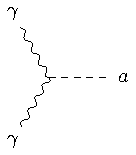
\includegraphics{diagrams/axion-biphoton.pdf}
	\hspace{4em}
	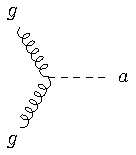
\includegraphics{diagrams/axion-bigluon.pdf}
	\caption{Axion--photon and axion-gluon interaction vertices.}
	\label{fig:axion-biphoton}
\end{figure}
The precise axion--matter interactions entering through the term $\LL_q'$ are model dependent, but generally have coupling strengths inversely proportional to the axion scale, $f_a$ \cite{Duffy_2009}.
However, all Peccei--Quinn axions interact with the gauge field though the last term in the Lagrangian \eqref{eqn:axion-Lagrangian}.
The last term is proportional to $\angbr{\tsbm F\wedge\tsbm F} = \ts F\wedge\ts F + \angbr{\tsbm G\wedge\tsbm G}$, where $\tsbm F = \ts F \oplus \tsbm G$ is the total gauge field decomposed into the electromagnetic $\ts F$ and gluonic $\tsbm G$ gauge fields.
In perturbation theory, this corresponds to a Feynman vertex in which an axion and two photons $aγγ$, or an axion and two gluons $agg$ meet, as in figure~\ref{fig:axion-biphoton}.
The $aγγ$ interaction is strong where $\ts F\wedge\ts F = (\bm E \cdot \bm B)\,\vol$ is large.
This implies that axions may be generated from photons, and vice-versa, in the presence of strong electromagnetic fields, suggesting methods for experimentally detecting axions in the lab or in astrophysical data.


\subsection{Axion Models}

\subsubsection{The Original Peccei--Quinn--Weinberg--Wilczek Axion}


The first proposed axion model, the Peccei--Quinn--Weinberg--Wilczek axion, \note{cite} implements the $\UPQ$ symmetry by supposing that the standard model possessed two Higgs fields $h_1$ and $h_2$ which couple differently to up and down quarks.
Denoting by $\bm ψ_\pm = \bm ψ_\pm^{(u)} \oplus \bm ψ_\pm^{(d)}$ the left- and right-handed quarks arranged into up-type and down-type parts, the two Higgs fields
\begin{align}
	\LL_\text{Yukawa} = \Re\qty(h_1 \bar{\bm ψ}_+ \mat m_u \bm ψ_-^{(u)} + h_2 \bar{\bm ψ}_+ \mat m_d \bm ψ_-^{(d)})
,\end{align}
where $\mat m_u$ and $\mat m_d$ are (non-square) matrices of Yukawa coupling constants.
The presence of the two Higgs fields lets $\LL_\text{Yukawa}$ be invariant under two independent chiral rotations of the up and down quarks, hence accomplishing the additional $\UPQ$ symmetry.

In this model, the axion scale is necessarily equal to the electroweak scale, $f_a \approx \SI{246}{\giga\eV}$.

\note{State that is physically excluded}

\subsubsection{Invisible Axions}

KSVZ (Kim--Shifman--Vainshtein--Zakharov)
DFSZ (Dine--Fischler--Srednicki--Zhitnitsky)